\emph{Pure Object Transaction} (POT) es la herramienta que implementa el
aspecto transaccional definido en la sección \ref{aspectoTransaccional}.
Está basada en una implementación anterior de Nicolás Passerini y Javier
Fernandes, que se actualizó para aprovechar el framework APO y facilitar su
integración con las demás herramientas desarrolladas.

\medskip
 
Este framework intercepta todas las lecturas y escrituras de los atributos de
un objeto, delegando tanto las lecturas como las escrituras al
\emph{administrador de las transacciones}.
A su vez, el administrador de transacciones asocia el pedido con un contexto
transaccional, que guarda los valores de los atributos de un objeto que fueron
modificados durante la transacción en una estructura de la forma
\code{[objeto, [nombre del atributo, valor]]}.
Cada contexto transaccional esta asociado a un \emph{thread}. Esto
permite manejar la concurrencia en el acceso a la información de los objetos.
Para aplicarle este aspecto a una clase se utiliza la \emph{annotation}.

\lstinline|Transactional|
	\begin{lstlisting} 
		@Transactional
		public class Client {
		}
	\end{lstlisting}
	
\medskip
 
La herramienta provee también soporte para transacciones anidadas.
Al momento de hacer el \emph{commit} en una transacción, los valores
contenidos en el contexto transaccional son impactados en la transacción
padre.
En caso de tratarse de una transacción de primer nivel, los cambios se impactan
en los objetos de dominio usando \emph{reflection}.
Esta forma de implementación permite que la identidad del objeto se
mantenga, ya que el objeto no se modifica ni se clona, solo se intercepta el
acceso a sus atributos.

Otro agregado a la versión original es la intersección de las modificaciones 
a un objeto de tipo \lstinline|Collection|, por ejemplo agregar o quitar
objetos de una colección.
Esto presenta un desafío especial ya que habitualmente en los programas Java
se utilizan las implementaciones de colecciones provistas por el propio
lenguaje y no es posible aplicar aspectos sobre estas clases. 
En la nueva versión, este problema se resuelve reemplazando en forma
automática las colecciones del lenguaje Java por
implementaciones propias de las mismas interfaces.
La figura \ref{potuml} muestra esquemáticamente el diseño de la herramienta.

\begin{figure}[!htbp]
	\centering
	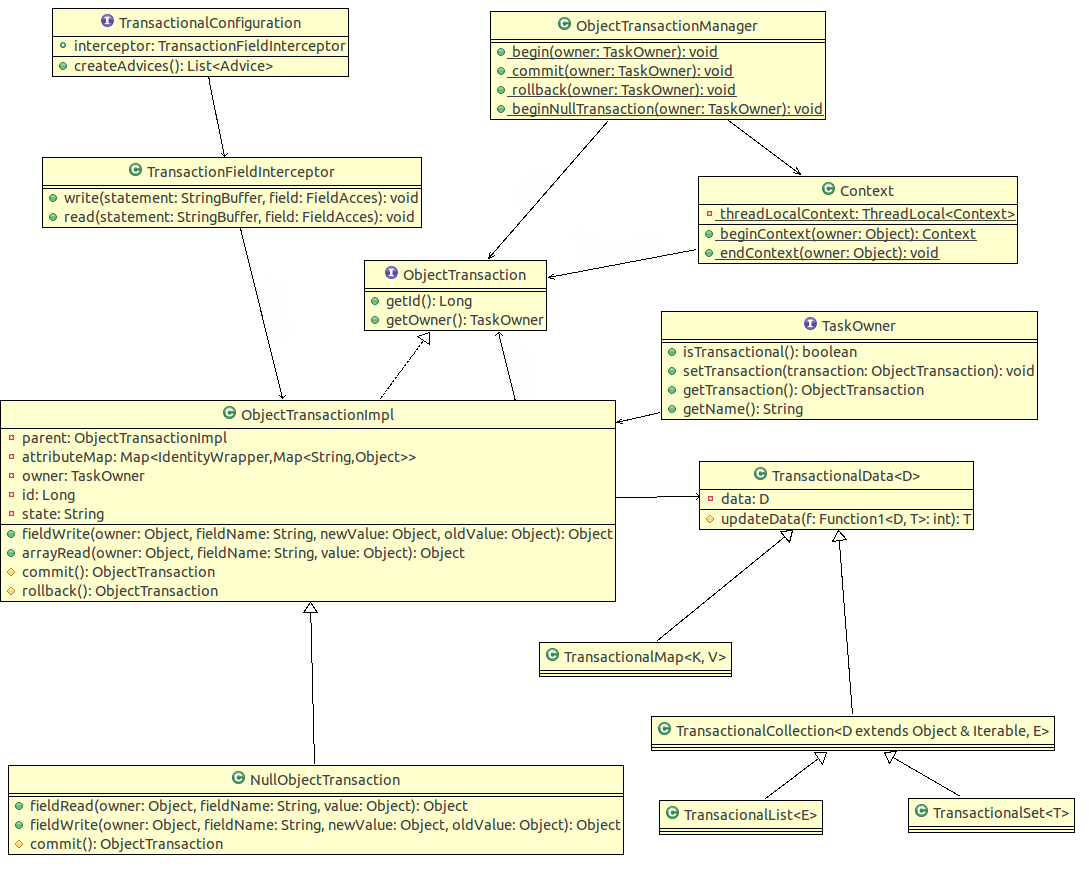
\includegraphics[scale=0.4]{img/pot}
 	\caption{Esquema de la herramienta POT}
 	\label{potuml}
\end{figure}
